\documentclass{ximera}

%\usepackage{todonotes}

\newcommand{\todo}{}

\usepackage{tkz-euclide}
\tikzset{>=stealth} %% cool arrow head
\tikzset{shorten <>/.style={ shorten >=#1, shorten <=#1 } } %% allows shorter vectors

\usepackage{tkz-tab}  %% sign charts
\usetikzlibrary{decorations.pathreplacing} 

\usetikzlibrary{backgrounds} %% for boxes around graphs
\usetikzlibrary{shapes,positioning}  %% Clouds and stars
\usetikzlibrary{matrix} %% for matrix
\usepgfplotslibrary{polar} %% for polar plots
\usetkzobj{all}
\usepackage[makeroom]{cancel} %% for strike outs
%\usepackage{mathtools} %% for pretty underbrace % Breaks Ximera
\usepackage{multicol}

\usepackage{polynom}



\usepackage[many]{tcolorbox}  %% for titled boxes
\newtcolorbox{xbox}[1]{%
    tikznode boxed title,
    enhanced,
    arc=0mm,
    interior style={white},
    attach boxed title to top center= {yshift=-\tcboxedtitleheight/2},
    fonttitle=\bfseries,
    colbacktitle=white,coltitle=black,
    boxed title style={size=normal,colframe=white,boxrule=0pt},
    title={#1}}


\usepackage{array}
\setlength{\extrarowheight}{+.1cm}   
\newdimen\digitwidth
\settowidth\digitwidth{9}
\def\divrule#1#2{
\noalign{\moveright#1\digitwidth
\vbox{\hrule width#2\digitwidth}}}





\newcommand{\RR}{\mathbb R}
\newcommand{\R}{\mathbb R}
\newcommand{\N}{\mathbb N}
\newcommand{\Z}{\mathbb Z}

%\renewcommand{\d}{\,d\!}
\renewcommand{\d}{\mathop{}\!d}
\newcommand{\dd}[2][]{\frac{\d #1}{\d #2}}
\newcommand{\pp}[2][]{\frac{\partial #1}{\partial #2}}
\renewcommand{\l}{\ell}
\newcommand{\ddx}{\frac{d}{\d x}}
\newcommand{\ddt}{\frac{d}{\d t}}

\newcommand{\zeroOverZero}{\ensuremath{\boldsymbol{\tfrac{0}{0}}}}
\newcommand{\inftyOverInfty}{\ensuremath{\boldsymbol{\tfrac{\infty}{\infty}}}}
\newcommand{\zeroOverInfty}{\ensuremath{\boldsymbol{\tfrac{0}{\infty}}}}
\newcommand{\zeroTimesInfty}{\ensuremath{\small\boldsymbol{0\cdot \infty}}}
\newcommand{\inftyMinusInfty}{\ensuremath{\small\boldsymbol{\infty - \infty}}}
\newcommand{\oneToInfty}{\ensuremath{\boldsymbol{1^\infty}}}
\newcommand{\zeroToZero}{\ensuremath{\boldsymbol{0^0}}}
\newcommand{\inftyToZero}{\ensuremath{\boldsymbol{\infty^0}}}



\newcommand{\numOverZero}{\ensuremath{\boldsymbol{\tfrac{\#}{0}}}}
\newcommand{\dfn}{\textbf}
%\newcommand{\unit}{\,\mathrm}
\newcommand{\unit}{\mathop{}\!\mathrm}
\newcommand{\eval}[1]{\bigg[ #1 \bigg]}
\newcommand{\seq}[1]{\left( #1 \right)}
\renewcommand{\epsilon}{\varepsilon}
\renewcommand{\iff}{\Leftrightarrow}

\DeclareMathOperator{\arccot}{arccot}
\DeclareMathOperator{\arcsec}{arcsec}
\DeclareMathOperator{\arccsc}{arccsc}
\DeclareMathOperator{\si}{Si}
\DeclareMathOperator{\proj}{proj}
\DeclareMathOperator{\scal}{scal}


\newcommand{\tightoverset}[2]{% for arrow vec
  \mathop{#2}\limits^{\vbox to -.5ex{\kern-0.75ex\hbox{$#1$}\vss}}}
\newcommand{\arrowvec}[1]{\tightoverset{\scriptstyle\rightharpoonup}{#1}}
\renewcommand{\vec}{\mathbf}
\newcommand{\veci}{\vec{i}}
\newcommand{\vecj}{\vec{j}}
\newcommand{\veck}{\vec{k}}
\newcommand{\vecl}{\boldsymbol{\l}}

\newcommand{\dotp}{\bullet}
\newcommand{\cross}{\boldsymbol\times}
\newcommand{\grad}{\boldsymbol\nabla}
\newcommand{\divergence}{\grad\dotp}
\newcommand{\curl}{\grad\cross}
%\DeclareMathOperator{\divergence}{divergence}
%\DeclareMathOperator{\curl}[1]{\grad\cross #1}


\colorlet{textColor}{black} 
\colorlet{background}{white}
\colorlet{penColor}{blue!50!black} % Color of a curve in a plot
\colorlet{penColor2}{red!50!black}% Color of a curve in a plot
\colorlet{penColor3}{red!50!blue} % Color of a curve in a plot
\colorlet{penColor4}{green!50!black} % Color of a curve in a plot
\colorlet{penColor5}{orange!80!black} % Color of a curve in a plot
\colorlet{fill1}{penColor!20} % Color of fill in a plot
\colorlet{fill2}{penColor2!20} % Color of fill in a plot
\colorlet{fillp}{fill1} % Color of positive area
\colorlet{filln}{penColor2!20} % Color of negative area
\colorlet{fill3}{penColor3!20} % Fill
\colorlet{fill4}{penColor4!20} % Fill
\colorlet{fill5}{penColor5!20} % Fill
\colorlet{gridColor}{gray!50} % Color of grid in a plot

\newcommand{\surfaceColor}{violet}
\newcommand{\surfaceColorTwo}{redyellow}
\newcommand{\sliceColor}{greenyellow}




\pgfmathdeclarefunction{gauss}{2}{% gives gaussian
  \pgfmathparse{1/(#2*sqrt(2*pi))*exp(-((x-#1)^2)/(2*#2^2))}%
}


%%%%%%%%%%%%%
%% Vectors
%%%%%%%%%%%%%

%% Simple horiz vectors
\renewcommand{\vector}[1]{\left\langle #1\right\rangle}


%% %% Complex Horiz Vectors with angle brackets
%% \makeatletter
%% \renewcommand{\vector}[2][ , ]{\left\langle%
%%   \def\nextitem{\def\nextitem{#1}}%
%%   \@for \el:=#2\do{\nextitem\el}\right\rangle%
%% }
%% \makeatother

%% %% Vertical Vectors
%% \def\vector#1{\begin{bmatrix}\vecListA#1,,\end{bmatrix}}
%% \def\vecListA#1,{\if,#1,\else #1\cr \expandafter \vecListA \fi}

%%%%%%%%%%%%%
%% End of vectors
%%%%%%%%%%%%%

%\newcommand{\fullwidth}{}
%\newcommand{\normalwidth}{}



%% makes a snazzy t-chart for evaluating functions
%\newenvironment{tchart}{\rowcolors{2}{}{background!90!textColor}\array}{\endarray}

%%This is to help with formatting on future title pages.
\newenvironment{sectionOutcomes}{}{} 



%% Flowchart stuff
%\tikzstyle{startstop} = [rectangle, rounded corners, minimum width=3cm, minimum height=1cm,text centered, draw=black]
%\tikzstyle{question} = [rectangle, minimum width=3cm, minimum height=1cm, text centered, draw=black]
%\tikzstyle{decision} = [trapezium, trapezium left angle=70, trapezium right angle=110, minimum width=3cm, minimum height=1cm, text centered, draw=black]
%\tikzstyle{question} = [rectangle, rounded corners, minimum width=3cm, minimum height=1cm,text centered, draw=black]
%\tikzstyle{process} = [rectangle, minimum width=3cm, minimum height=1cm, text centered, draw=black]
%\tikzstyle{decision} = [trapezium, trapezium left angle=70, trapezium right angle=110, minimum width=3cm, minimum height=1cm, text centered, draw=black]


\outcome{Solve basic related rates word problems.}
\outcome{Understand the process of solving related rates problems.}
\outcome{Calculate derivatives of expressions with multiple variables implicitly.}

\title[Dig-In:]{More than one rate}

\begin{document}
	\begin{abstract}
		Here we work abstract related rates problems.
	\end{abstract}
	\maketitle
	
	
	Suppose we have two, variables $x$ and $y$, which are both changing with
	respect to time.  A \textit{related rates} problem is a problem where
	we know one rate, say $\frac{dx}{dt}$, at a given instant, and wish to find the other (the unknown rate is "related" to the known rate).
	
	Here, the chain rule is key: If $y$ is written in terms of $x$, and we
	are given $\dd[x]{t}$, then it is easy to find $\dd[y]{t}$ using the
	chain rule:
	\[
	y=y(x)
	\]
	\[
	\dd[y]{t}=\dd[y]{x}\cdot \dd[x]{t}.
	\]
	In many cases, particularly the interesting ones, our functions will
	be related in some other way. Nevertheless, in each case we'll use the
	chain rule to help us find the desired rate. In this
	section, we will work several abstract examples in order to emphasize
	the mathematical concepts involved. In each of the examples below, we
	will follow essentially the same plan of attack:
	
	
	
	\begin{description}
		\item[\textbf{Introduce variables, identify the given rate and the unknown rate.}]
		
		Assign a variable to each quantity that changes in time.
		\item[\textbf{Draw a picture.}] If possible, draw a schematic picture with all the relevant information. 
		\item[\textbf{Find equations.}] Write equations that relate all
		relevant variables.
		\item[\textbf{Differentiate with respect to t.}] Here we will often use
		implicit differentiation and obtain an equation that relates the given rate and the unknown rate. 
		\item[\textbf{Evaluate and solve.}] Evaluate
		each quantity at the relevant instant and solve for the unknown rate.
		
	\end{description}
	
	
	
	
	\section{Formulas}
	
	In order to relate several variables we can use known formulas.
	
	In our next example we consider an expanding circle and use the formulas for perimeter and area of a circle.
	
	\begin{image}
		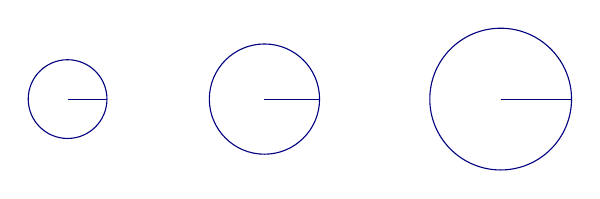
\begin{tikzpicture}
		\draw [penColor] (-3,0) circle [radius=0.5];
		\draw [penColor] (-0.5,0) circle [radius=0.7];
		\draw [penColor] (2.5,0) circle [radius=0.9];
		\draw [penColor] (-3,0) -- (-2.5,0);
		\draw [penColor] (-0.5,0) -- (0.2,0);
		\draw [penColor] (2.5,0) -- (3.4,0);
		\end{tikzpicture}
	\end{image}
	\begin{example}
		Imagine an expanding circle. If we know that the perimeter is
		expanding at a rate of $4$ m/s, at what rate is the area changing
		when the radius is $3$ meters?
		\begin{explanation}
			
			
			
			First, we \textbf{introduce the variables} $P$, $r$, and $A$,  denoting the perimeter, the radius, and  the area of the circle, in that order. 
			
			We \textbf{identify} the given rate, $\frac{dP}{dt}=4$ m/s, and the unknown rate, $\frac{dA}{dt}$, at the moment when $r=3$. 
			
			Next, we \textbf{draw a picture}.
			\begin{image}
				\begin{tikzpicture}
				\draw [penColor, very thick] (0,0) circle [radius=2];
				\draw [penColor] (0,0) -- (2,0);
				\node [below,penColor] at (1,0) {$r$ };
				\node [penColor,left] at (4.6,1.02) {$\dfrac{dP}{dt}= 4$ m/s};
				\node [penColor2,left] at (5.99,-0.2) {$\frac{dA}{dt} = $ ? , when $r=3$ };
				
				\end{tikzpicture}
			\end{image}
			Now we have to \textbf{find equations} that relate
			the variables $P$, $r$, and $A$. 
			
			Naturally, we think of formulas for perimeter and area of a circle
			\[
			P = 2\cdot \pi \cdot \answer[given]{r}
			\qquad\text{and}\qquad
			A = \pi \cdot \answer[given]{r^{2}}.
			\]
			We know that the perimeter of the circle is expanding. This implies that both the radius and the area of the circle are changing in time, too.
			So, we note that $P$, $r$, and $A$ are functions of time
			\[
			P(t) = 2\cdot \pi \cdot r(t)
			\qquad\text{and}\qquad
			A(t) = \pi \cdot r(t)^2.
			\]
			We \textbf{differentiate} both sides of each equation with respect to time, $t$.  Using implicit
			differentiation, we get that
			
			\[
			\underbrace{ \dfrac{d}{dt}P(t)}_{given\hspace{0.05in} rate} = 2\cdot \pi\cdot  \dfrac{d}{dt}r(t)
			\qquad\text{and}\qquad
			\underbrace{ \dfrac{d}{dt}A(t)}_{unknown \hspace{0.05in}rate} = 2\cdot \pi\cdot r(t) \cdot  \dfrac{d}{dt}r(t).
			\]
			
			These two equations hold on some time interval. In particular, they are both true at an instant when $r=3$.
			
			We know  that at that instant $ \dfrac{d}{dt}P(t) =
			\answer[given]{4}$ and $r = \answer[given]{3}$. 
			
			We now \textbf{evaluate}  the two equations at the instant when $r=3$.
			
			\[
			4 = 2\cdot \pi\cdot \dfrac{d}{dt}r(t)
			\qquad\text{and}\qquad
			\dfrac{d}{dt}A(t) = 2\cdot \pi\cdot 3 \cdot \dfrac{d}{dt}r(t) 
			\]
			
			
			From the first equation we get that
			\begin{align*}
				\dd{t}r(t)&=  2/\pi \hspace{0.1in} m/s, \hspace{0.1in} when \hspace{0.1in} r=3.    
			\end{align*} 
			
			Using this result and the equation on the right, we get, at the instant when $r=3$,
			
			\begin{align*}
				\dfrac{d}{dt}A(t) &= 2\cdot \pi\cdot 3 \cdot 2/\pi\\
				&=\answer[given]{12}\hspace{0.1in} m^2/s.
			\end{align*}
			Hence, the area is expanding at a rate of $12$ $m^2/s$ at the instant when $r=3$ m.
		\end{explanation}
	\end{example}
	
	
	%%BADBAD
	%% There are a number of common formulas that arise in related rates
	%% problems.
	%%
	%% It might be nice to add a little list of common area/volume formulas.
	
	
	
	\section{Right triangles}
	
	
	In our next example, we consider an expanding right triangle and use the Pythagorean Theorem to relate relevant variables.
	\begin{image}
		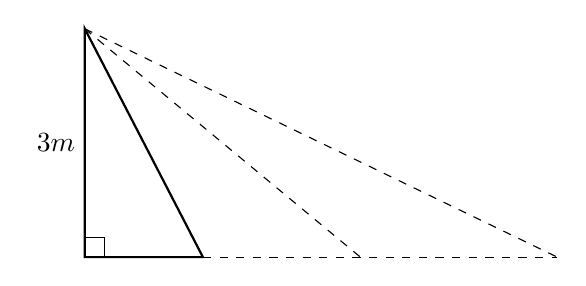
\begin{tikzpicture}
		\coordinate (A) at (0,0);
		\coordinate (B) at (0,2.9);
		\coordinate (C) at (1.5,0);
		\coordinate (D) at (3.5,0);
		\coordinate (E) at (6,0);
		\tkzMarkRightAngle(C,A,B)
		\tkzDefMidPoint(A,B) \tkzGetPoint{3 m}
		\tkzDefMidPoint(A,C) \tkzGetPoint{b}
		\tkzDefMidPoint(B,C) \tkzGetPoint{c}
		\draw [thick](A)--(B)--(C)--cycle;
		\draw[dashed](B)--(D);
		\draw[dashed](B)--(E);
		\draw[dashed](C)--(E);
		\tkzLabelPoints[left](3 m)
		%\tkzLabelPoints[left](a)
		
		\end{tikzpicture}
	\end{image}
	
	\begin{example}
		Imagine an expanding right triangle. If one leg has a fixed length
		of $3$ m, one leg is increasing with a rate of $2$ m/s, and the
		hypotenuse is expanding to accommodate the expanding leg, at what
		rate is the hypotenuse expanding when both legs are $3$ m long?
		\begin{explanation}
			First, we \textbf{introduce the variables}  $a$, $b$, and $c$, denoting the fixed length, the length of a leg that is increasing, 
			and  the length of the hypotenuse, in that order. Then, we \textbf{identify} the given rate $\frac{db}{dt}=2$ m/s and the unknown rate $\frac{dc}{dt}$, when $b=3$.
			Now, we \textbf{draw a picture}.
			\begin{image}
				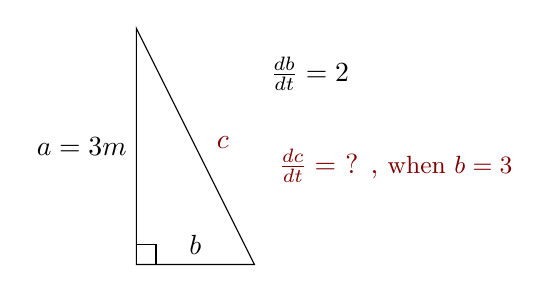
\begin{tikzpicture}
				\coordinate (A) at (0,0);
				\coordinate (B) at (0,3);
				\coordinate (C) at (1.5,0);
				\tkzMarkRightAngle(C,A,B)
				\tkzDefMidPoint(A,B) \tkzGetPoint{a}
				\tkzDefMidPoint(A,C) \tkzGetPoint{b}
				\tkzDefMidPoint(B,C) \tkzGetPoint{c}
				\draw (A)--(B)--(C)--cycle;
				
				\tkzLabelPoints[above](b)
				\node [penColor2] at (1.1,1.55){$c$};
				%\tkzLabelPoints[left](a)
				\node [left] at (a) {$a = 3 m$};
				\node at (2.2,2.42){$\frac{db}{dt} = 2$};
				\node [penColor2,left] at (4.9,1.25) {$\frac{dc}{dt} = $ ? , \small{when $b=3$} };
				\end{tikzpicture}
			\end{image}
			
			Next, we  \textbf{find equations} that relate relevant
			variables. Here we use the Pythagorean Theorem.
			\[
			c^2 = a^2 + b^2
			\]
			Note that $a=3$ is a constant, and $c$ and $b$ are functions of time, $t$.
			We, then, \textbf{differentiate} both sides of the equation with respect to $t$,  using  implicit differentiation
			
			\[
			2\cdot c(t)\cdot\dfrac{d}{dt}c(t) = 2\cdot b\cdot\dfrac{d}{dt}b(t).
			\]
			Now, we \textbf{evaluate} all the quantities at the instant when $b=3$, noting that
			$\dfrac{db}{dt} = 2$ and that $b = 3$. Therefore,
			\[
			2\cdot c\cdot\dfrac{dc}{dt}= \answer[given]{12},\hspace{0.08in} when\hspace{0.08in}b=3.
			\]
			We need to compute $c$, the length of the hypotenuse at the instant when $b=3$. Here we use
			the Pythagorean Theorem
			\begin{align*}
				c^2 &= 3^2 + 3^2\\
				&=\answer[given]{18},
			\end{align*}
			So, we see that $c = 3\sqrt{2}$, when $b=3$. \\
			Then, we \textbf{solve} for the rate at the moment when $b=3$,\\
			\begin{align*}
				6\sqrt{2}\cdot \dfrac{dc}{dt} &= 12 \\     
				\dfrac{dc}{dt} &= \sqrt{2}.
			\end{align*}
			Therefore, the hypotenuse  is growing at a rate of $\answer[given]{\sqrt{2}}$ m/s when both legs are $3m$ long.
		\end{explanation}
	\end{example}
	
	
	\section{Angular rates}
	
	
	We can also investigate problems involving angular rates.
	
	\begin{example}
		Imagine an expanding right triangle. If one leg has a fixed length
		of $3$ m, one leg is increasing with a rate of $2$ m/s, and the
		hypotenuse is expanding to accommodate the expanding leg, at what
		rate is the angle opposite the fixed leg changing when both legs
		are $3$ m long?
		\begin{explanation}
			First, we \textbf{introduce the variables}  $a$, $b$, $c$, as in the previous example, and $\theta$, denoting
			the angle opposite the leg with fixed length. 
			
			
			We \textbf{identify} the given rate $\frac{db}{dt}=2$ m/s and the unknown rate $\frac{d\theta}{dt}$, when $b=3$.
			
			
			Next, we \textbf{draw a picture}.
			\begin{image}
				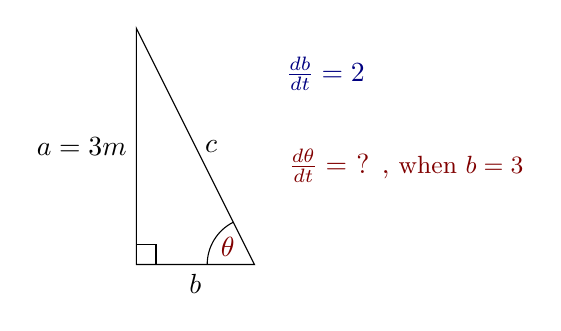
\begin{tikzpicture}
				\coordinate (A) at (0,0);
				\coordinate (B) at (0,3);
				\coordinate (C) at (1.5,0);
				\tkzMarkRightAngle(C,A,B)
				\tkzDefMidPoint(A,B) \tkzGetPoint{a}
				\tkzDefMidPoint(A,C) \tkzGetPoint{b}
				\tkzDefMidPoint(B,C) \tkzGetPoint{c}
				\draw (A)--(B)--(C)--cycle;
				\tkzLabelPoints[right](c)
				
				\tkzMarkAngle[size=0.6cm,thin](B,C,A)
				
				%\tkzLabelPoints[left](a)
				\node [left] at (a) {$a = 3 m$};
				\node [below] at (b) {$b$};
				\node [penColor2] at (1.16,0.22){$\theta$};
				\node [penColor] at (2.4,2.42){$\frac{db}{dt} = 2$};
				\node [penColor2,left] at (5.04,1.25) {$\frac{d\theta}{dt} = $ ? , \small{when $b=3$} };
				\end{tikzpicture}
			\end{image}
			
			
			We now \textbf{find equations} that combine relevant
			variables. Here we note that
			\[
			\tan(\theta) = \frac{3}{\answer[given]{b}}.
			\]
			Since $\theta$ and $b$ are functions of time, we
			\textbf{differentiate}  both sides of  the equation using
			implicit differentiation
			
			\[
			\sec^2(\theta)\frac{d\theta}{dt} = \frac{-3}{b^2}\cdot \frac{db}{dt}.
			\]
			Now, we \textbf{evaluate} all the quantities at the instant when $b=3$, keeping in mind that
			$\frac{db}{dt} = 2$ and $b = 3$,
			\[
			\sec^2(\theta)\cdot\dfrac{d\theta}{dt}= \frac{-3}{3^2}\cdot 2\\
			= \frac{-2}{3} .
			\]
			It is clear that we still need to compute $ \sec^2(\theta)$ at the moment when $b=3$. A picture will help.
			\begin{image}
				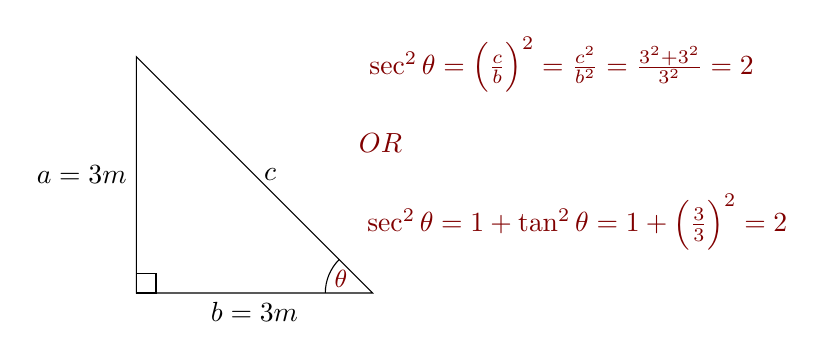
\begin{tikzpicture}
				\coordinate (A) at (0,0);
				\coordinate (B) at (0,3);
				\coordinate (C) at (3,0);
				\tkzMarkRightAngle(C,A,B)
				\tkzDefMidPoint(A,B) \tkzGetPoint{a}
				\tkzDefMidPoint(A,C) \tkzGetPoint{b}
				\tkzDefMidPoint(B,C) \tkzGetPoint{c}
				\draw (A)--(B)--(C)--cycle;
				\tkzLabelPoints[right](c)
				
				\tkzMarkAngle[size=0.6cm,thin](B,C,A)
				
				%\tkzLabelPoints[left](a)
				\node [left] at (a) {$a = 3 m$};
				\node [below] at (b) {$b=3 m$};
				\node [penColor2] at (2.6,0.18){\small$\theta$};
				\node [penColor2] at (5.4,2.9){$\sec^2{\theta}=\Bigl(\frac{c}{b}\Bigr)^2=\frac{c^2}{b^2}=\frac{3^2+3^2}{3^2}=2$};
				\node [penColor2] at (3.1,1.9){$OR$};
				\node [penColor2] at (5.6,0.9){$\sec^2{\theta}=1+\tan^2{\theta}=1+\Bigl(\frac{3}{3}\Bigr)^2=2$};
				\end{tikzpicture}
			\end{image}
			
			Since we know the lengths of both legs in the right triangle, it is easier to compute
			
			$\tan(\theta)$ than  $\sec(\theta)$. Recall the trig identity:  $ \sec^2(\theta)=1+  \tan^2(\theta)$.
			\begin{align*}
				\sec^2(\theta)&= 1+ \tan^2(\theta)\\
				&= 1+\Bigl(\frac{3}{3}\Bigr)^2\\
				&= \answer[given]{2}
			\end{align*}
			Now we \textbf{solve} for the unknown rate, when $b=3$,
			\begin{align*}
				2\cdot \dfrac{d\theta}{dt} &= \frac{-2}{3}\\
				\dfrac{d\theta}{dt}&= \frac{-1}{3}
			\end{align*}
			So, when $b=3$, the angle is changing at $\answer[given]{-1/3}$
			radians per second.
		\end{explanation}
	\end{example}
	
	
	
	\section{Similar triangles}
	
	Finally, facts about similar triangles are often useful when solving
	related rates problems.
	
	\begin{example}
		The figure shows two right triangles that share an (acute) angle. 
		\begin{image}
			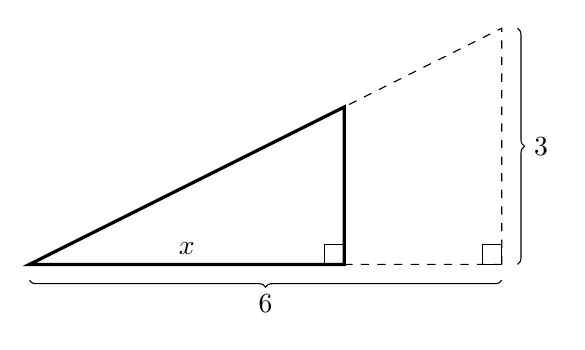
\begin{tikzpicture}
			\coordinate (A) at (6,2);
			\coordinate (B) at (6,5);
			\coordinate (C) at (0,2);
			\coordinate (D) at (4,2);
			\coordinate (E) at (4,4);
			\tkzMarkRightAngle(C,A,B)
			\tkzMarkRightAngle(C,D,E)
			\tkzDefMidPoint(A,B) \tkzGetPoint{a}
			\tkzDefMidPoint(A,C) \tkzGetPoint{b}
			\tkzDefMidPoint(D,C) \tkzGetPoint{x}
			\draw[decoration={brace,mirror,raise=.2cm},decorate,thin] (0,2)--(6,2);
			\draw[decoration={brace,mirror,raise=.2cm},decorate,thin] (6,2)--(6,5);
			\draw[dashed] (A)--(B)--(C)--cycle;
			\draw[very thick] (D)--(E)--(C)--cycle;
			\tkzLabelPoints[above](x)
			\node at (3,2-.5) {$6$};
			\node at (6+.5,3.5) {$3$};
			\end{tikzpicture}
		\end{image}
		If $x$ is growing from the vertex with a rate of $3$ m/s, what rate
		is the area of the smaller triangle changing when $x = 5$m?
		\begin{explanation}
			First, we \textbf{introduce the variables} $h$ and $A$, denoting the height and the area of the smaller triangle, in that order.
			Next, we \textbf{identify} the given rate $\frac{dx}{dt}=3$ m/s and the unknown rate $\frac{dA}{dt}$, when $x=5$.
			Despite the fact that a nice picture is given, we should do what
			we always do and \textbf{draw a picture}. Note, we ad
			information to the picture:
			\begin{image}
				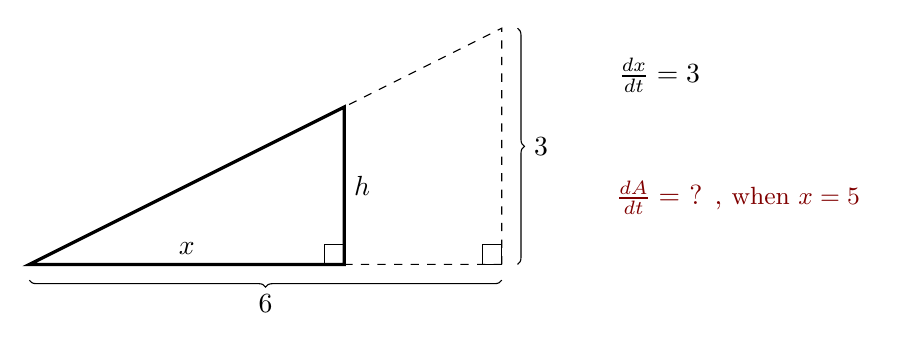
\begin{tikzpicture}
				\coordinate (A) at (6,2);
				\coordinate (B) at (6,5);
				\coordinate (C) at (0,2);
				\coordinate (D) at (4,2);
				\coordinate (E) at (4,4);
				\tkzMarkRightAngle(C,A,B)
				\tkzMarkRightAngle(C,D,E)
				\tkzDefMidPoint(A,B) \tkzGetPoint{a}
				\tkzDefMidPoint(A,C) \tkzGetPoint{b}
				\tkzDefMidPoint(D,C) \tkzGetPoint{x}
				\tkzDefMidPoint(D,E) \tkzGetPoint{h}
				\draw[decoration={brace,mirror,raise=.2cm},decorate,thin] (0,2)--(6,2);
				\draw[decoration={brace,mirror,raise=.2cm},decorate,thin] (6,2)--(6,5);
				\draw[dashed] (A)--(B)--(C)--cycle;
				\draw[very thick] (D)--(E)--(C)--cycle;
				\tkzLabelPoints[above](x)
				\tkzLabelPoints[right](h)
				\node at (3,2-.5) {$6$};
				\node at (6+.5,3.5) {$3$};
				\node at (8,4.4) {$\frac{dx}{dt}=3$};
				\node [penColor2] at (9,2.85) {$\frac{dA}{dt}=$ ? , \small{when $x=5$} };
				\end{tikzpicture}
			\end{image}
			
			
			Next, we \textbf{find equations} that combine relevant
			variables. In this case there are two. The first is the formula
			for the area of a triangle:
			\[
			A = \frac{1}{2} \cdot x \cdot h
			\]
			The second uses the fact that the larger triangle is similar to
			the smaller triangle, meaning that the ratios between the corresponding sides in both triangles
			are equal,
			\[
			\frac{h}{x} = \frac{3}{\answer[given]{6}}\qquad\text{so}\qquad h =
			\frac{1}{\answer[given]{2}}\cdot x
			\]
			At this point we could \textbf{differentiate} both equations, but we 
			choose a simpler path and express  $A$ in terms of $x$  
			\begin{align*}
				A& = \frac{1}{2} \cdot x\cdot\underbrace{ \frac{1}{2}\cdot x}_{h} .
			\end{align*}
			
			Therefore,
			\[
			A=\frac{1}{4}\cdot x^2.
			\]
			Since $A$ and $x$ are both functions of time, we \textbf{differentiate} both sides of this equation with respect to $t$
			
			\[
			\frac{dA}{dt}=\frac{1}{4}\cdot2\cdot x\cdot\frac{dx}{dt}.
			\]
			In particular, when $x=5$, 
			\[
			\frac{dA}{dt}=\frac{1}{4}\cdot2\cdot 5\cdot 3=\answer{\frac{15}{2}}.
			\]
			
			Hence, the area is changing at a rate of $ \frac{15}{2}$ $\text{m}^2/\text{s}$ when $x=5$m.
			
		\end{explanation}
	\end{example}
\end{document}
